%\clearpage
\section{System}\label{sec:Schluss}
\subsubsection{Zugangsdaten}
In der nachfolgenden Tabelle sind die Zugangsdaten, welche in diesem Projekt verwendet wurden.

\begin{table}[H]
	\centering
	\begin{tabular}{|l|l|l|l|}
		\hline 
		Dienst & Benutzername & Passwort & IP-Adresse \\ 
		\hline 
		WLAN & LA7722 & 490f2490 &  \\ 
		\hline 
		Openhab & openhabian & openhabian & 192.168.137.8 \\ 
		\hline 
		Home Assistant & uuserdue & uuserdue &  \\ 
		\hline 
		Cloud Nabu Casa & Uuserdue@gmail.com&uuserdue&\\
		\hline
	\end{tabular} 
\end{table}
\subsubsection{Systemübersicht}
   \begin{figure}[H]
	\centering
	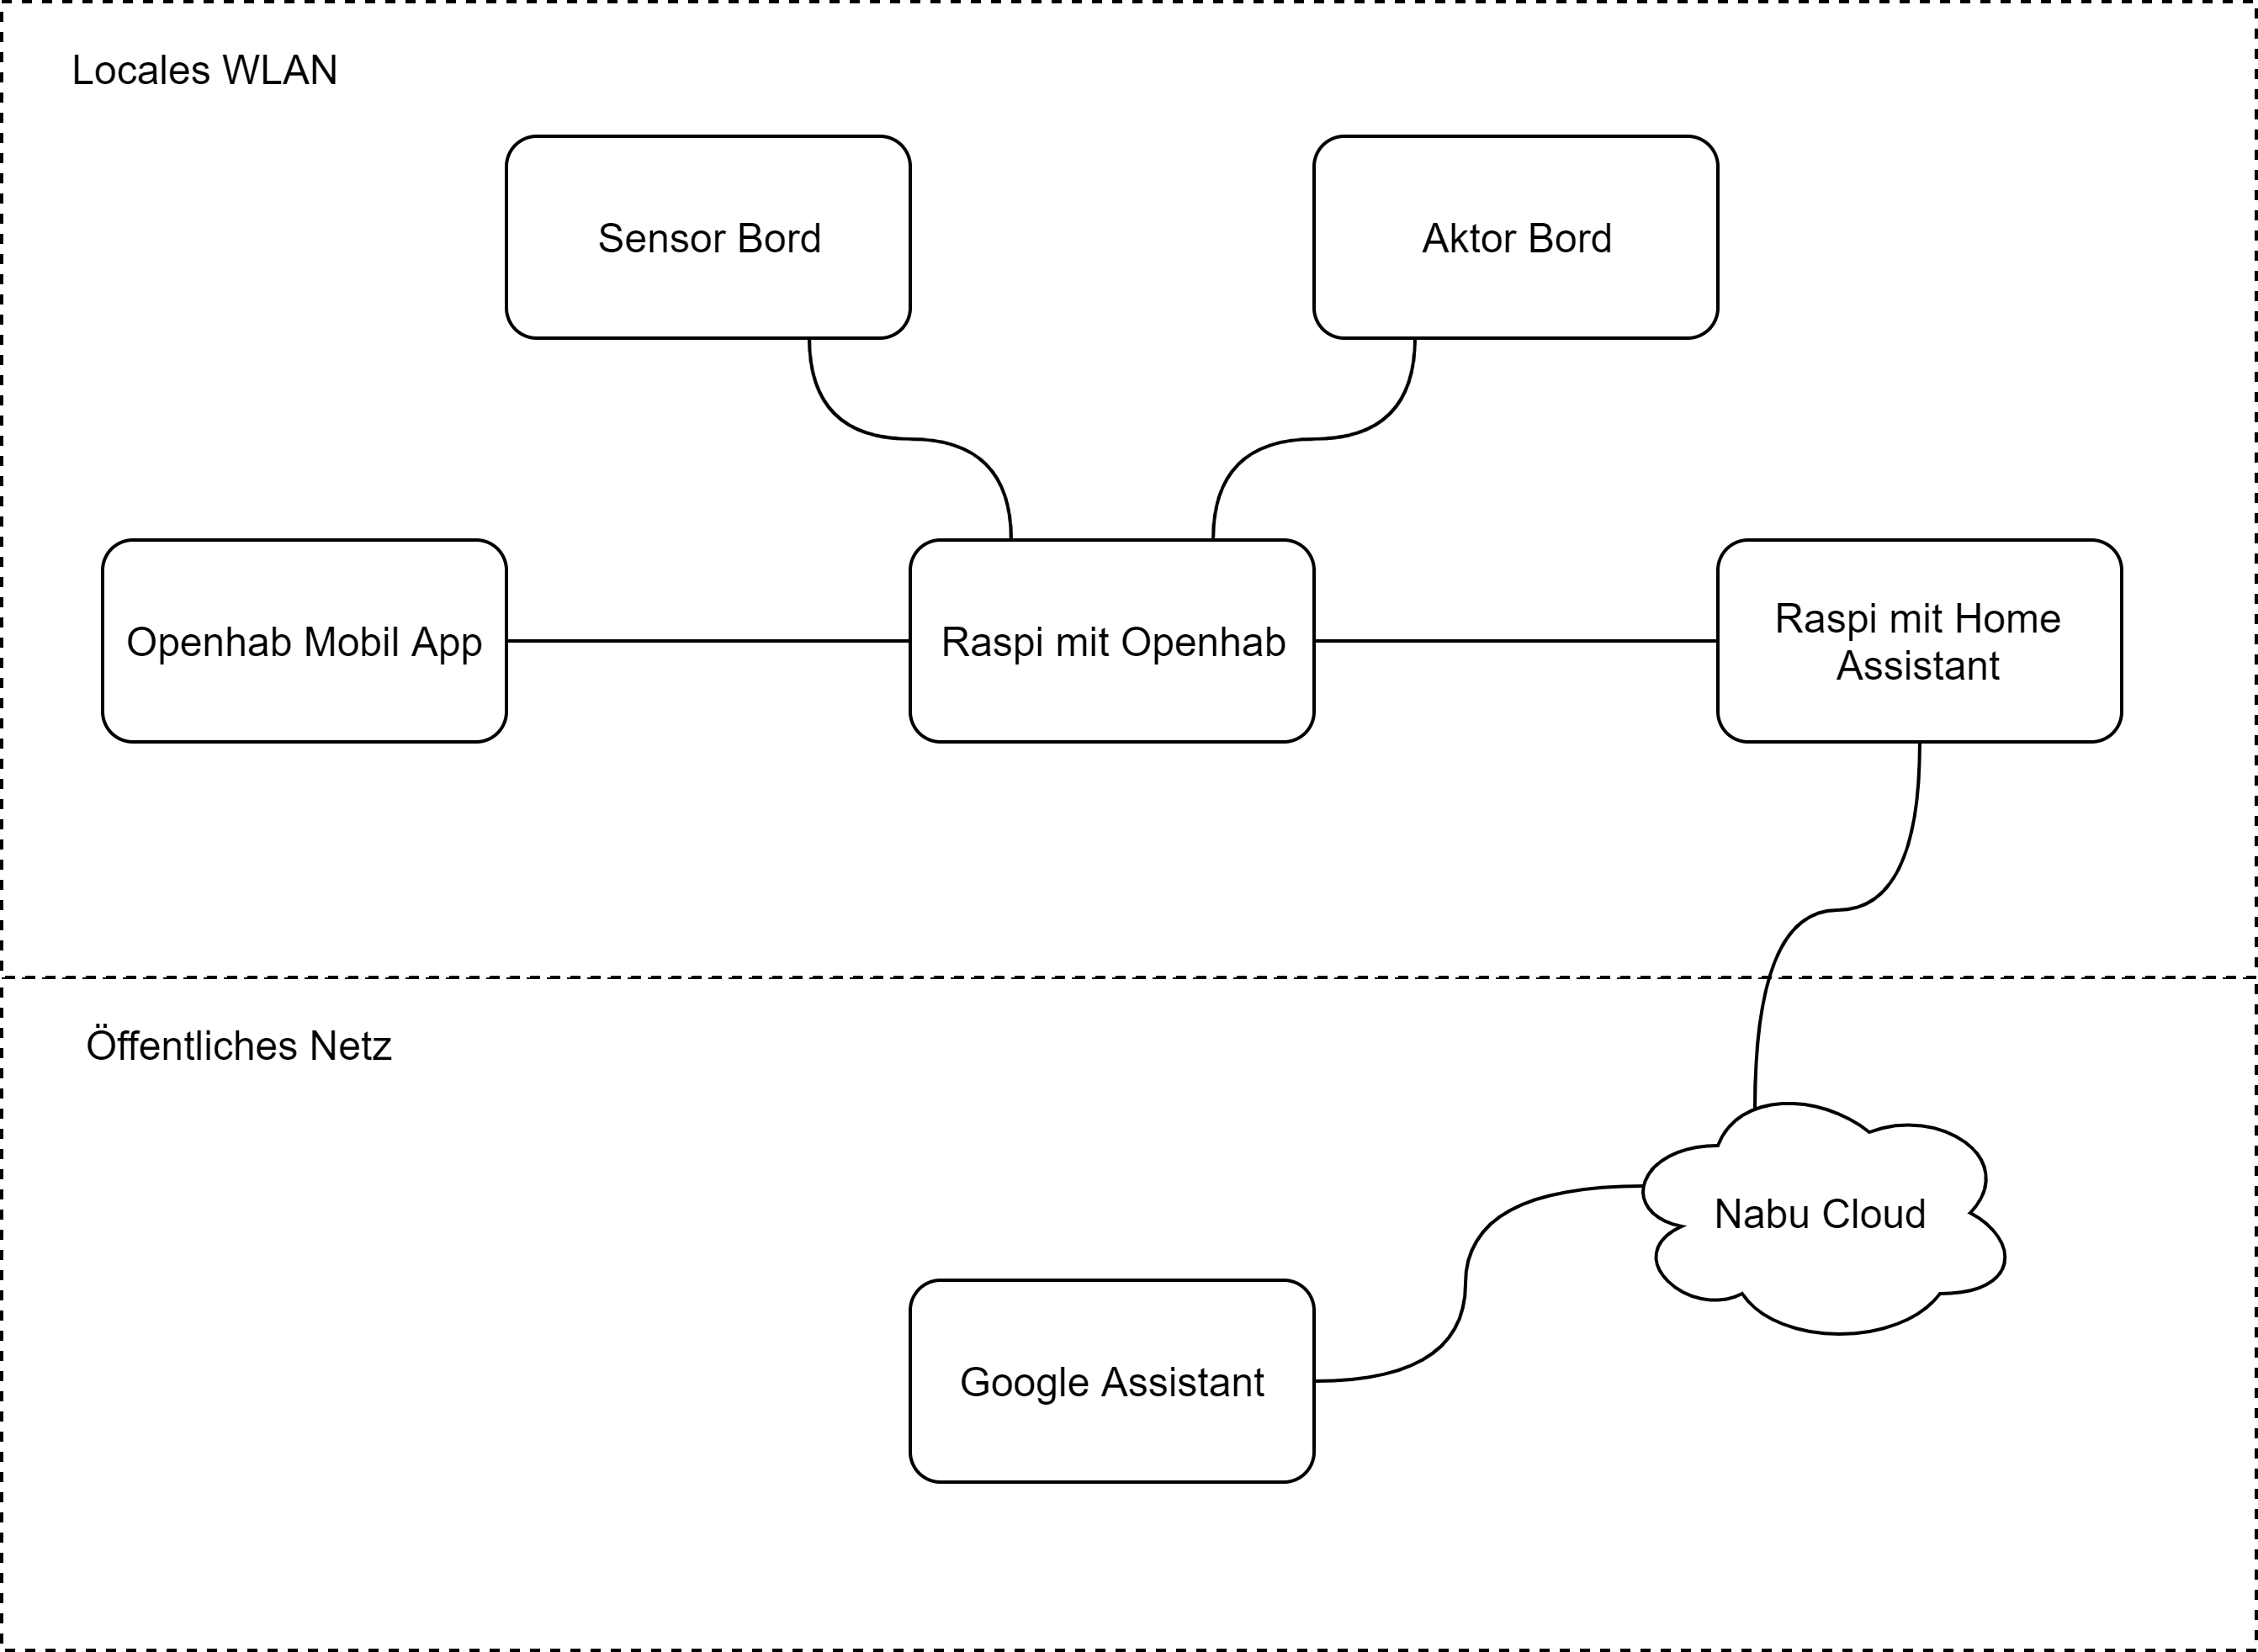
\includegraphics[width=\textwidth]{graphics/Systemubersicht.png}
	\caption{Systemübersicht} 	
	\label{pic: Systemübersicht}
\end{figure}
In der Systemübersicht ist zu erkennen, dass das gesamte System im lokalen Netz Funktioniert mit der Ausnahme vom Sprachassistent. Dies erhöht die Zuverlässigkeit und die Sicherheit der Smart-Home Lösung. 




